\section{Sommario}

Abbiamo messo a punto un sistema di rivelazione \emph{multi-purpose} adatto al volo su pallone. Per soddisfare le richieste tecniche ed effettuare tutte le misure di nostro interesse, l'esperimento sfrutta elettronica \emph{ad hoc} e rivelatori alla frontiera tecnologica sviluppati dall'INFN. Prima dell'eventuale lancio il sistema verr\'a testato da noi in laboratorio: questa potr\'a essere per noi l'occasione di condurre un esperimento di fisica delle particelle, seguendolo in tutte le fasi, dalla progettazione fino all'analisi dati. Le sfide di questo progetto richiedono la collaborazione tra diverse aree del sapere scientifico, permettendoci di uscire dai nostri ambiti specifici e arricchendoci col lavoro comune.

\begin{figure}[h]
\centering
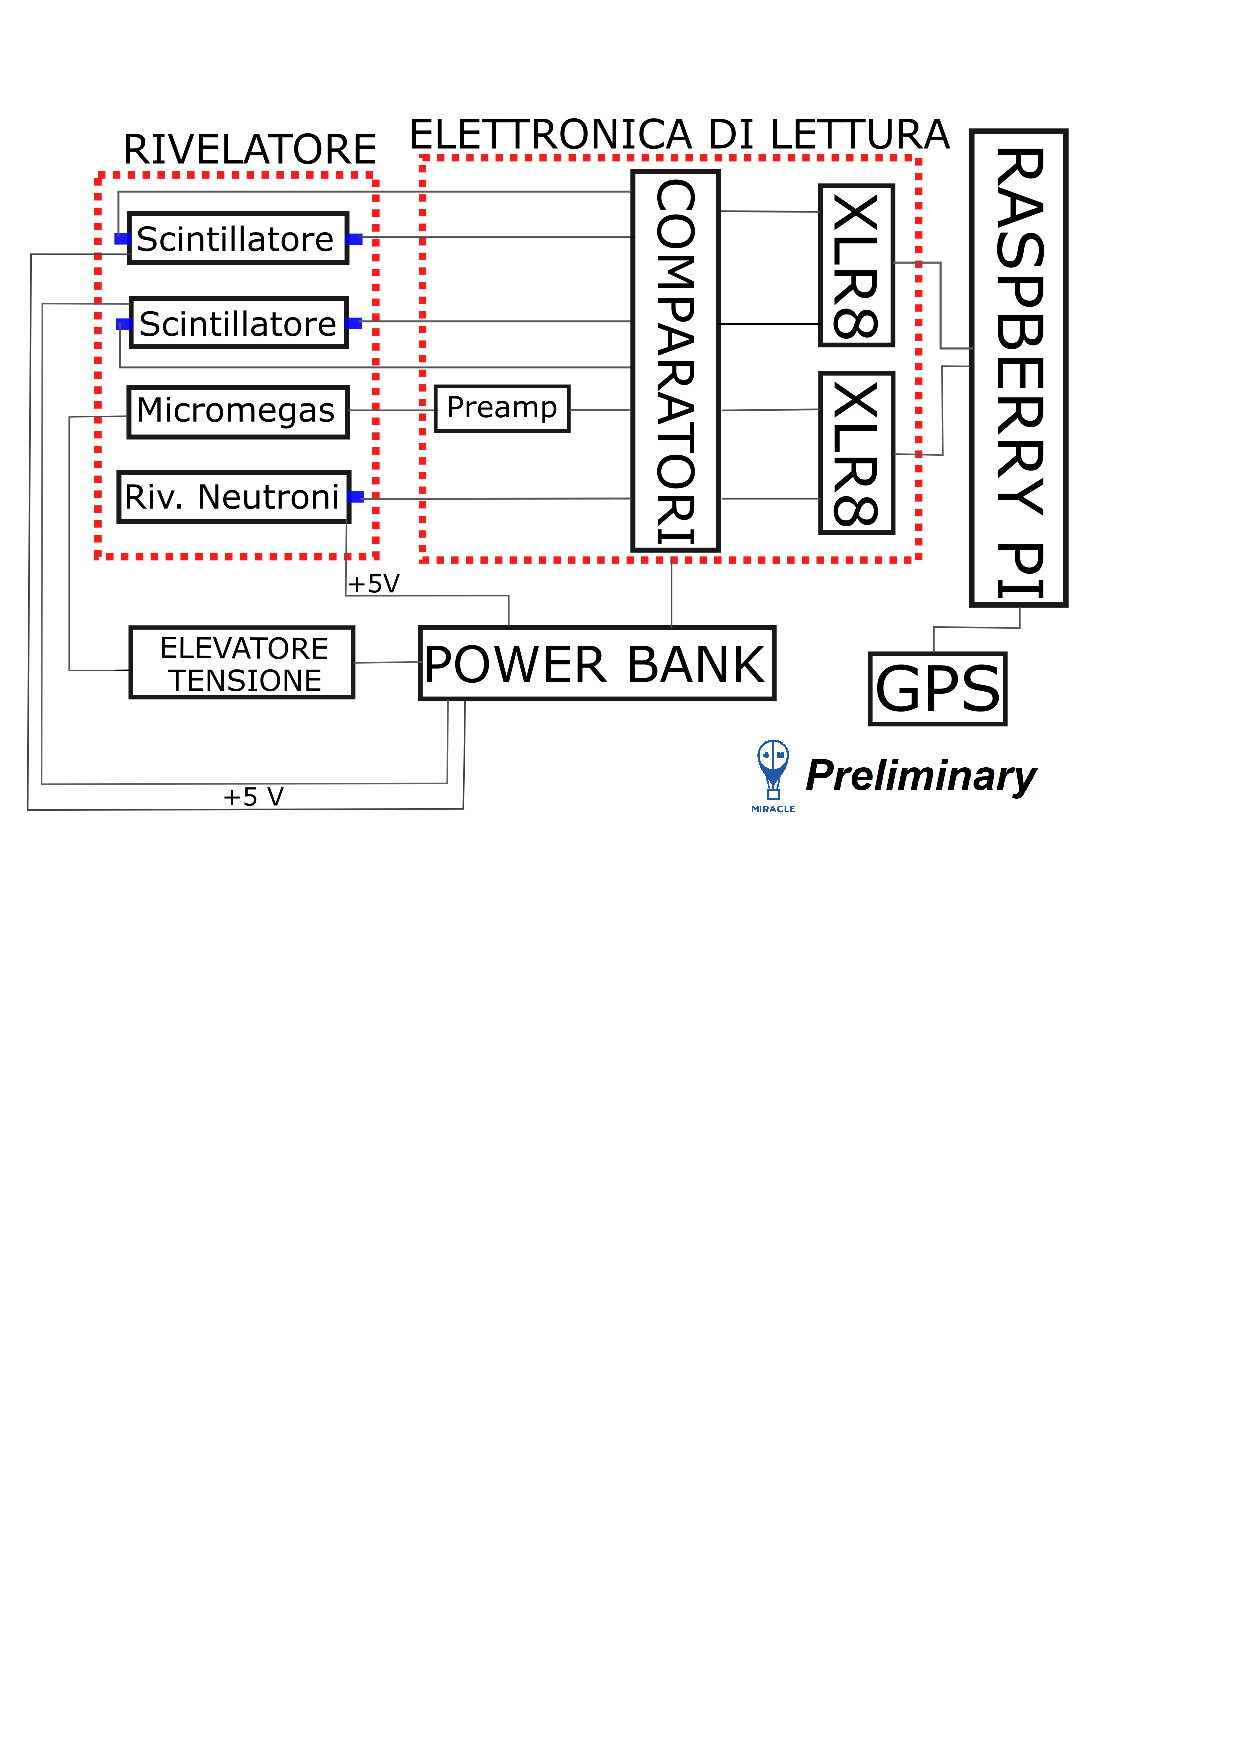
\includegraphics[width=0.5\textwidth]{SCHEMATICA.pdf}
\caption{Schematica riassuntiva dell'apparato rivelatore, dell'elettronica Front-End e dell'elettronica di acquisizioni dati.}
\label{schematica}
\end{figure}
